\documentclass[twoside]{book}

% Packages required by doxygen
\usepackage{fixltx2e}
\usepackage{calc}
\usepackage{doxygen}
\usepackage[export]{adjustbox} % also loads graphicx
\usepackage{graphicx}
\usepackage[utf8]{inputenc}
\usepackage{makeidx}
\usepackage{multicol}
\usepackage{multirow}
\PassOptionsToPackage{warn}{textcomp}
\usepackage{textcomp}
\usepackage[nointegrals]{wasysym}
\usepackage[table]{xcolor}

% Font selection
\usepackage[T1]{fontenc}
\usepackage[scaled=.90]{helvet}
\usepackage{courier}
\usepackage{amssymb}
\usepackage{sectsty}
\renewcommand{\familydefault}{\sfdefault}
\allsectionsfont{%
  \fontseries{bc}\selectfont%
  \color{darkgray}%
}
\renewcommand{\DoxyLabelFont}{%
  \fontseries{bc}\selectfont%
  \color{darkgray}%
}
\newcommand{\+}{\discretionary{\mbox{\scriptsize$\hookleftarrow$}}{}{}}

% Page & text layout
\usepackage{geometry}
\geometry{%
  a4paper,%
  top=2.5cm,%
  bottom=2.5cm,%
  left=2.5cm,%
  right=2.5cm%
}
\tolerance=750
\hfuzz=15pt
\hbadness=750
\setlength{\emergencystretch}{15pt}
\setlength{\parindent}{0cm}
\setlength{\parskip}{3ex plus 2ex minus 2ex}
\makeatletter
\renewcommand{\paragraph}{%
  \@startsection{paragraph}{4}{0ex}{-1.0ex}{1.0ex}{%
    \normalfont\normalsize\bfseries\SS@parafont%
  }%
}
\renewcommand{\subparagraph}{%
  \@startsection{subparagraph}{5}{0ex}{-1.0ex}{1.0ex}{%
    \normalfont\normalsize\bfseries\SS@subparafont%
  }%
}
\makeatother

% Headers & footers
\usepackage{fancyhdr}
\pagestyle{fancyplain}
\fancyhead[LE]{\fancyplain{}{\bfseries\thepage}}
\fancyhead[CE]{\fancyplain{}{}}
\fancyhead[RE]{\fancyplain{}{\bfseries\leftmark}}
\fancyhead[LO]{\fancyplain{}{\bfseries\rightmark}}
\fancyhead[CO]{\fancyplain{}{}}
\fancyhead[RO]{\fancyplain{}{\bfseries\thepage}}
\fancyfoot[LE]{\fancyplain{}{}}
\fancyfoot[CE]{\fancyplain{}{}}
\fancyfoot[RE]{\fancyplain{}{\bfseries\scriptsize Generated by Doxygen }}
\fancyfoot[LO]{\fancyplain{}{\bfseries\scriptsize Generated by Doxygen }}
\fancyfoot[CO]{\fancyplain{}{}}
\fancyfoot[RO]{\fancyplain{}{}}
\renewcommand{\footrulewidth}{0.4pt}
\renewcommand{\chaptermark}[1]{%
  \markboth{#1}{}%
}
\renewcommand{\sectionmark}[1]{%
  \markright{\thesection\ #1}%
}

% Indices & bibliography
\usepackage{natbib}
\usepackage[titles]{tocloft}
\setcounter{tocdepth}{3}
\setcounter{secnumdepth}{5}
\makeindex

% Hyperlinks (required, but should be loaded last)
\usepackage{ifpdf}
\ifpdf
  \usepackage[pdftex,pagebackref=true]{hyperref}
\else
  \usepackage[ps2pdf,pagebackref=true]{hyperref}
\fi
\hypersetup{%
  colorlinks=true,%
  linkcolor=blue,%
  citecolor=blue,%
  unicode%
}

% Custom commands
\newcommand{\clearemptydoublepage}{%
  \newpage{\pagestyle{empty}\cleardoublepage}%
}

\usepackage{caption}
\captionsetup{labelsep=space,justification=centering,font={bf},singlelinecheck=off,skip=4pt,position=top}

%===== C O N T E N T S =====

\begin{document}

% Titlepage & ToC
\hypersetup{pageanchor=false,
             bookmarksnumbered=true,
             pdfencoding=unicode
            }
\pagenumbering{alph}
\begin{titlepage}
\vspace*{7cm}
\begin{center}%
{\Large Heap Helper }\\
\vspace*{1cm}
{\large Generated by Doxygen 1.8.13}\\
\end{center}
\end{titlepage}
\clearemptydoublepage
\pagenumbering{roman}
\tableofcontents
\clearemptydoublepage
\pagenumbering{arabic}
\hypersetup{pageanchor=true}

%--- Begin generated contents ---
\chapter{Class Index}
\section{Class List}
Here are the classes, structs, unions and interfaces with brief descriptions\+:\begin{DoxyCompactList}
\item\contentsline{section}{\hyperlink{structHeap}{Heap} }{\pageref{structHeap}}{}
\item\contentsline{section}{\hyperlink{structNode}{Node} }{\pageref{structNode}}{}
\end{DoxyCompactList}

\chapter{Class Documentation}
\hypertarget{structHeap}{}\section{Heap Struct Reference}
\label{structHeap}\index{Heap@{Heap}}


{\ttfamily \#include $<$heaphelper.\+h$>$}



Collaboration diagram for Heap\+:\nopagebreak
\begin{figure}[H]
\begin{center}
\leavevmode
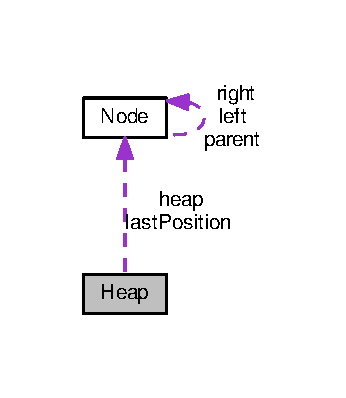
\includegraphics[width=166pt]{structHeap__coll__graph}
\end{center}
\end{figure}
\subsection*{Public Attributes}
\begin{DoxyCompactItemize}
\item 
\mbox{\Hypertarget{structHeap_a4f01a49a784cfda0ac4b0abd95a4ac06}\label{structHeap_a4f01a49a784cfda0ac4b0abd95a4ac06}} 
\hyperlink{structNode}{Node} $\ast$ \hyperlink{structHeap_a4f01a49a784cfda0ac4b0abd95a4ac06}{heap}
\begin{DoxyCompactList}\small\item\em contains all of the heap nodes \end{DoxyCompactList}\item 
\mbox{\Hypertarget{structHeap_a687e85d124c882bb01f5c9bf91171129}\label{structHeap_a687e85d124c882bb01f5c9bf91171129}} 
H\+E\+A\+P\+\_\+\+T\+Y\+PE \hyperlink{structHeap_a687e85d124c882bb01f5c9bf91171129}{type}
\begin{DoxyCompactList}\small\item\em flag for choosing between min and max heap \end{DoxyCompactList}\item 
\mbox{\Hypertarget{structHeap_a016750f22dcb8be0fd9cde478d270dd5}\label{structHeap_a016750f22dcb8be0fd9cde478d270dd5}} 
\hyperlink{structNode}{Node} $\ast$ \hyperlink{structHeap_a016750f22dcb8be0fd9cde478d270dd5}{last\+Position}
\begin{DoxyCompactList}\small\item\em optional element useful for finding where to insert the next value \end{DoxyCompactList}\item 
\mbox{\Hypertarget{structHeap_abc8d0107b18de7599058485d78c2e244}\label{structHeap_abc8d0107b18de7599058485d78c2e244}} 
void($\ast$ \hyperlink{structHeap_abc8d0107b18de7599058485d78c2e244}{destroy\+Data} )(void $\ast$data)
\begin{DoxyCompactList}\small\item\em function pointer to a function to delete a single piece of data from the heap \end{DoxyCompactList}\item 
\mbox{\Hypertarget{structHeap_a6f4d91e7eebe5e20d5ee60418c59c5e6}\label{structHeap_a6f4d91e7eebe5e20d5ee60418c59c5e6}} 
void($\ast$ \hyperlink{structHeap_a6f4d91e7eebe5e20d5ee60418c59c5e6}{print\+Node} )(void $\ast$to\+Be\+Printed)
\begin{DoxyCompactList}\small\item\em function pointer to a function that prints out a data element of the heap \end{DoxyCompactList}\item 
\mbox{\Hypertarget{structHeap_ab11468cee0bf82183a92cf2fa8bab107}\label{structHeap_ab11468cee0bf82183a92cf2fa8bab107}} 
int($\ast$ \hyperlink{structHeap_ab11468cee0bf82183a92cf2fa8bab107}{compare} )(const void $\ast$first, const void $\ast$second)
\begin{DoxyCompactList}\small\item\em function pointer to a comparison function for the purpose of inserting and deleting elements \end{DoxyCompactList}\item 
\mbox{\Hypertarget{structHeap_ac291cf589f86e95198621d33e21a05a6}\label{structHeap_ac291cf589f86e95198621d33e21a05a6}} 
int {\bfseries size}
\end{DoxyCompactItemize}


\subsection{Detailed Description}
\hyperlink{structHeap}{Heap} structure for binary tree implementation of a \hyperlink{structHeap}{Heap} 

The documentation for this struct was generated from the following file\+:\begin{DoxyCompactItemize}
\item 
include/heaphelper.\+h\end{DoxyCompactItemize}

\hypertarget{structNode}{}\section{Node Struct Reference}
\label{structNode}\index{Node@{Node}}


{\ttfamily \#include $<$Hash\+Table\+A\+P\+I.\+h$>$}



Collaboration diagram for Node\+:
\nopagebreak
\begin{figure}[H]
\begin{center}
\leavevmode
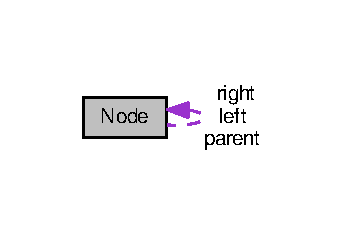
\includegraphics[width=160pt]{structNode__coll__graph}
\end{center}
\end{figure}
\subsection*{Public Attributes}
\begin{DoxyCompactItemize}
\item 
\mbox{\Hypertarget{structNode_ad88c9a757bfafd5ff265e0837b150056}\label{structNode_ad88c9a757bfafd5ff265e0837b150056}} 
char $\ast$ \hyperlink{structNode_ad88c9a757bfafd5ff265e0837b150056}{key}
\begin{DoxyCompactList}\small\item\em integer that represents a piece of data in the table (eg 35-\/$>$\char`\"{}hello\char`\"{}) \end{DoxyCompactList}\item 
\mbox{\Hypertarget{structNode_a38b733496e3eff5e0b4fcb11cd9b866a}\label{structNode_a38b733496e3eff5e0b4fcb11cd9b866a}} 
void $\ast$ \hyperlink{structNode_a38b733496e3eff5e0b4fcb11cd9b866a}{data}
\begin{DoxyCompactList}\small\item\em pointer to generic data that is to be stored in the hash table \end{DoxyCompactList}\item 
\mbox{\Hypertarget{structNode_af67b110ca1a258b793bf69d306929b22}\label{structNode_af67b110ca1a258b793bf69d306929b22}} 
struct \hyperlink{structNode}{Node} $\ast$ \hyperlink{structNode_af67b110ca1a258b793bf69d306929b22}{next}
\begin{DoxyCompactList}\small\item\em pointer to the next \hyperlink{structNode}{Node} if a collision is detected \end{DoxyCompactList}\end{DoxyCompactItemize}


\subsection{Detailed Description}
\hyperlink{structNode}{Node} of the hash table. 

The documentation for this struct was generated from the following file\+:\begin{DoxyCompactItemize}
\item 
include/\hyperlink{HashTableAPI_8h}{Hash\+Table\+A\+P\+I.\+h}\end{DoxyCompactItemize}

%--- End generated contents ---

% Index
\backmatter
\newpage
\phantomsection
\clearemptydoublepage
\addcontentsline{toc}{chapter}{Index}
\printindex

\end{document}
